\chapter{Test plan}\label{ch:test}
For the verification of the correctness of our implementation of
\cordic{} is to write a \matlab{} model of the algorithm and then compare the
output to the VHDL one.

\section{Floating Point Model}\label{sec:floating_point_model}
The first model we have to write is a floating point version of \cordic{}
algorithm as we can see in \lstref{lst:cordicfloatmatlab}.


\lstinputlisting[language=matlab, label={lst:cordicfloatmatlab},
caption={CORDIC Floating Point Model in Matlab 
(\code{cordic\_vectoring\_float.m}).}]{matlab/float/cordic_vectoring_float.m}

From this model we can obtain a measure of the algorithmic error, comparing the 
output of this algorithm, produced with a test input dataset\footnote{The test 
input dataset is composed by points lying on circumferences with different 
radius}, and compared to the radius and phase computed in "traditional" way.

The result is that both on phase and radius the error after 14 iterations is in
the order of \(10^{-8}\) for the radius in \figref{fig:floaterrorradius} and 
\(10^{-4}\) for the phase \figref{fig:floaterrorphase}. The resulting Mean
Square Errors and Max Errors are:

\[MSE_r = 2.8876\times10^{-18}\]
\[MSE_p = 4.2575\times10^{-9}\]
\[MaxError_r = 6.3350\times10^{-9}\]
\[MaxError_p = 1.1865\times10^{-4}\]


\begin{figure}[ht]
	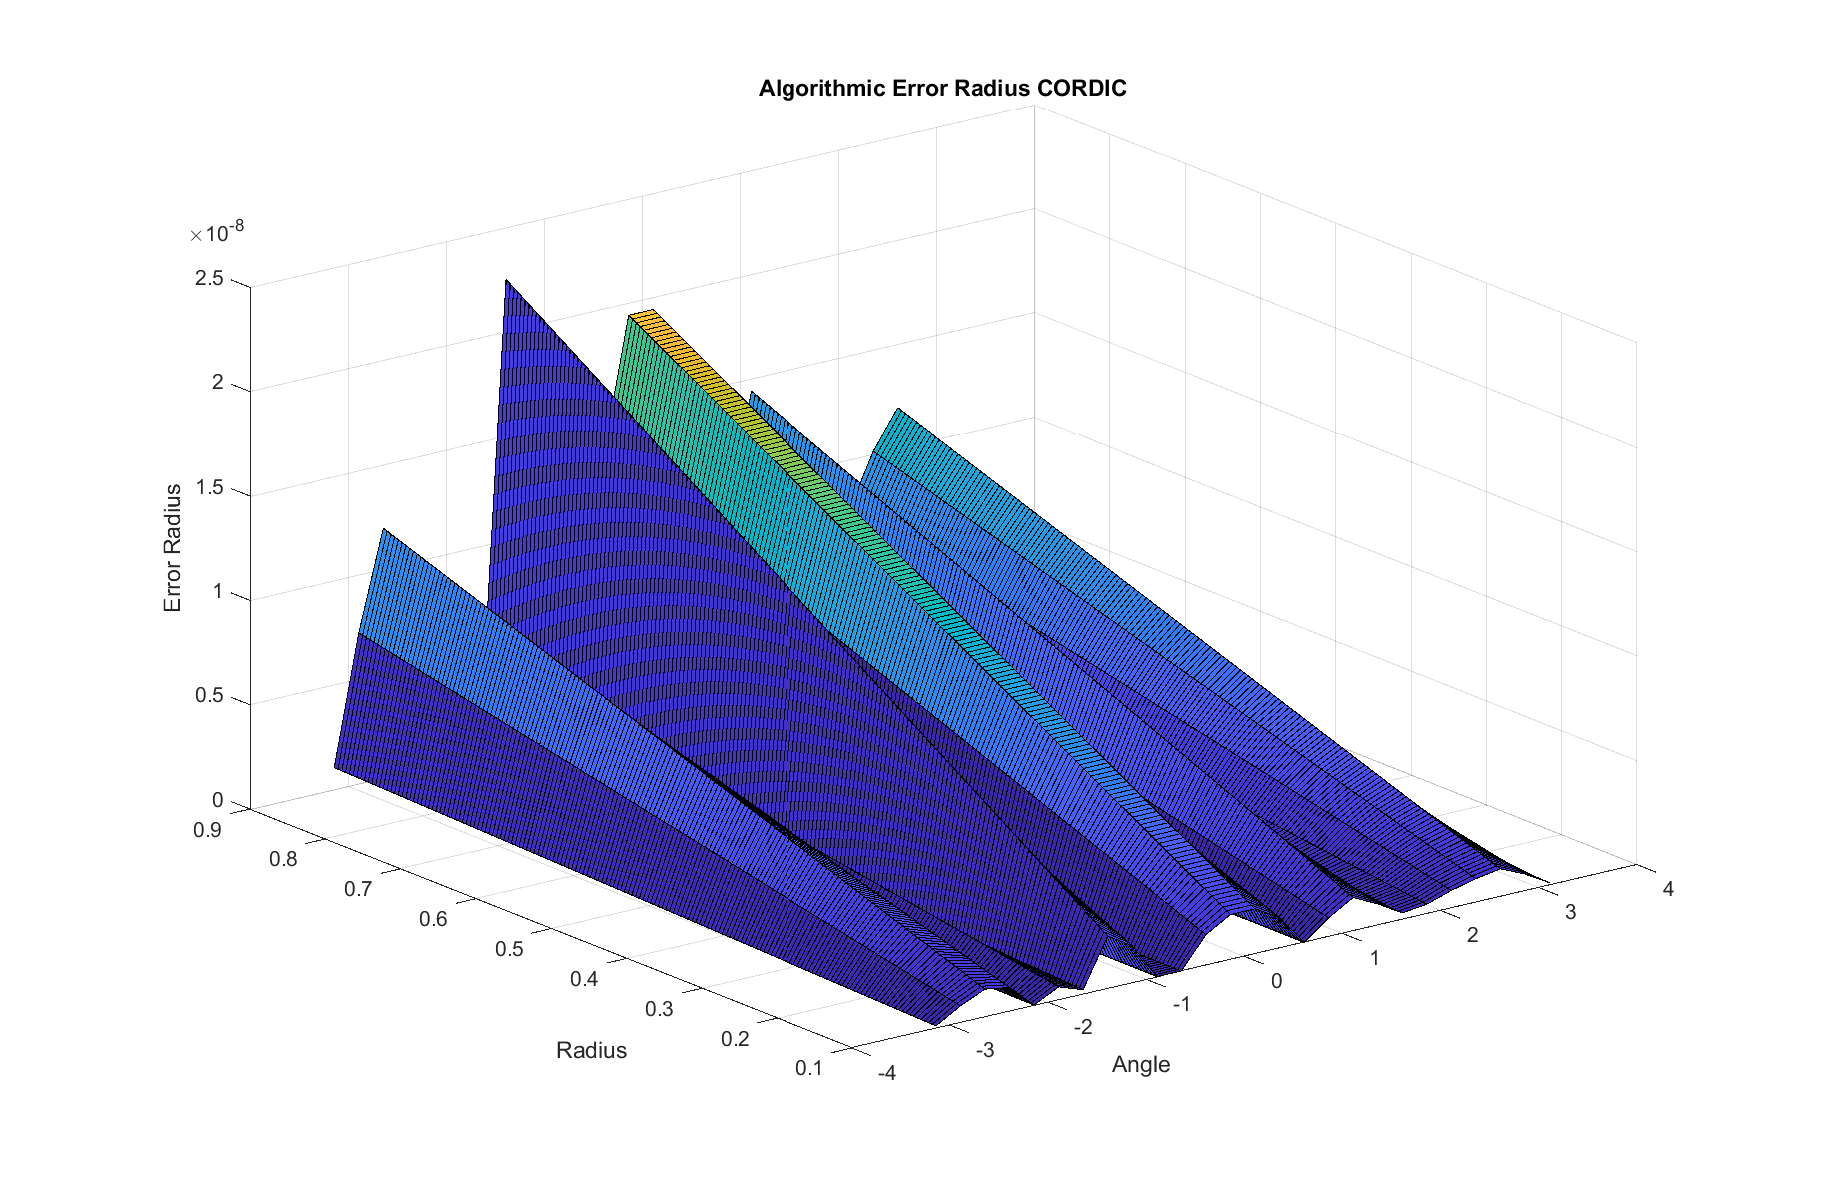
\includegraphics[width=\textwidth]{alg_error_radius}
	\caption{Algorithmic error Radius}\label{fig:floaterrorradius}
\end{figure}
\begin{figure}[ht]
	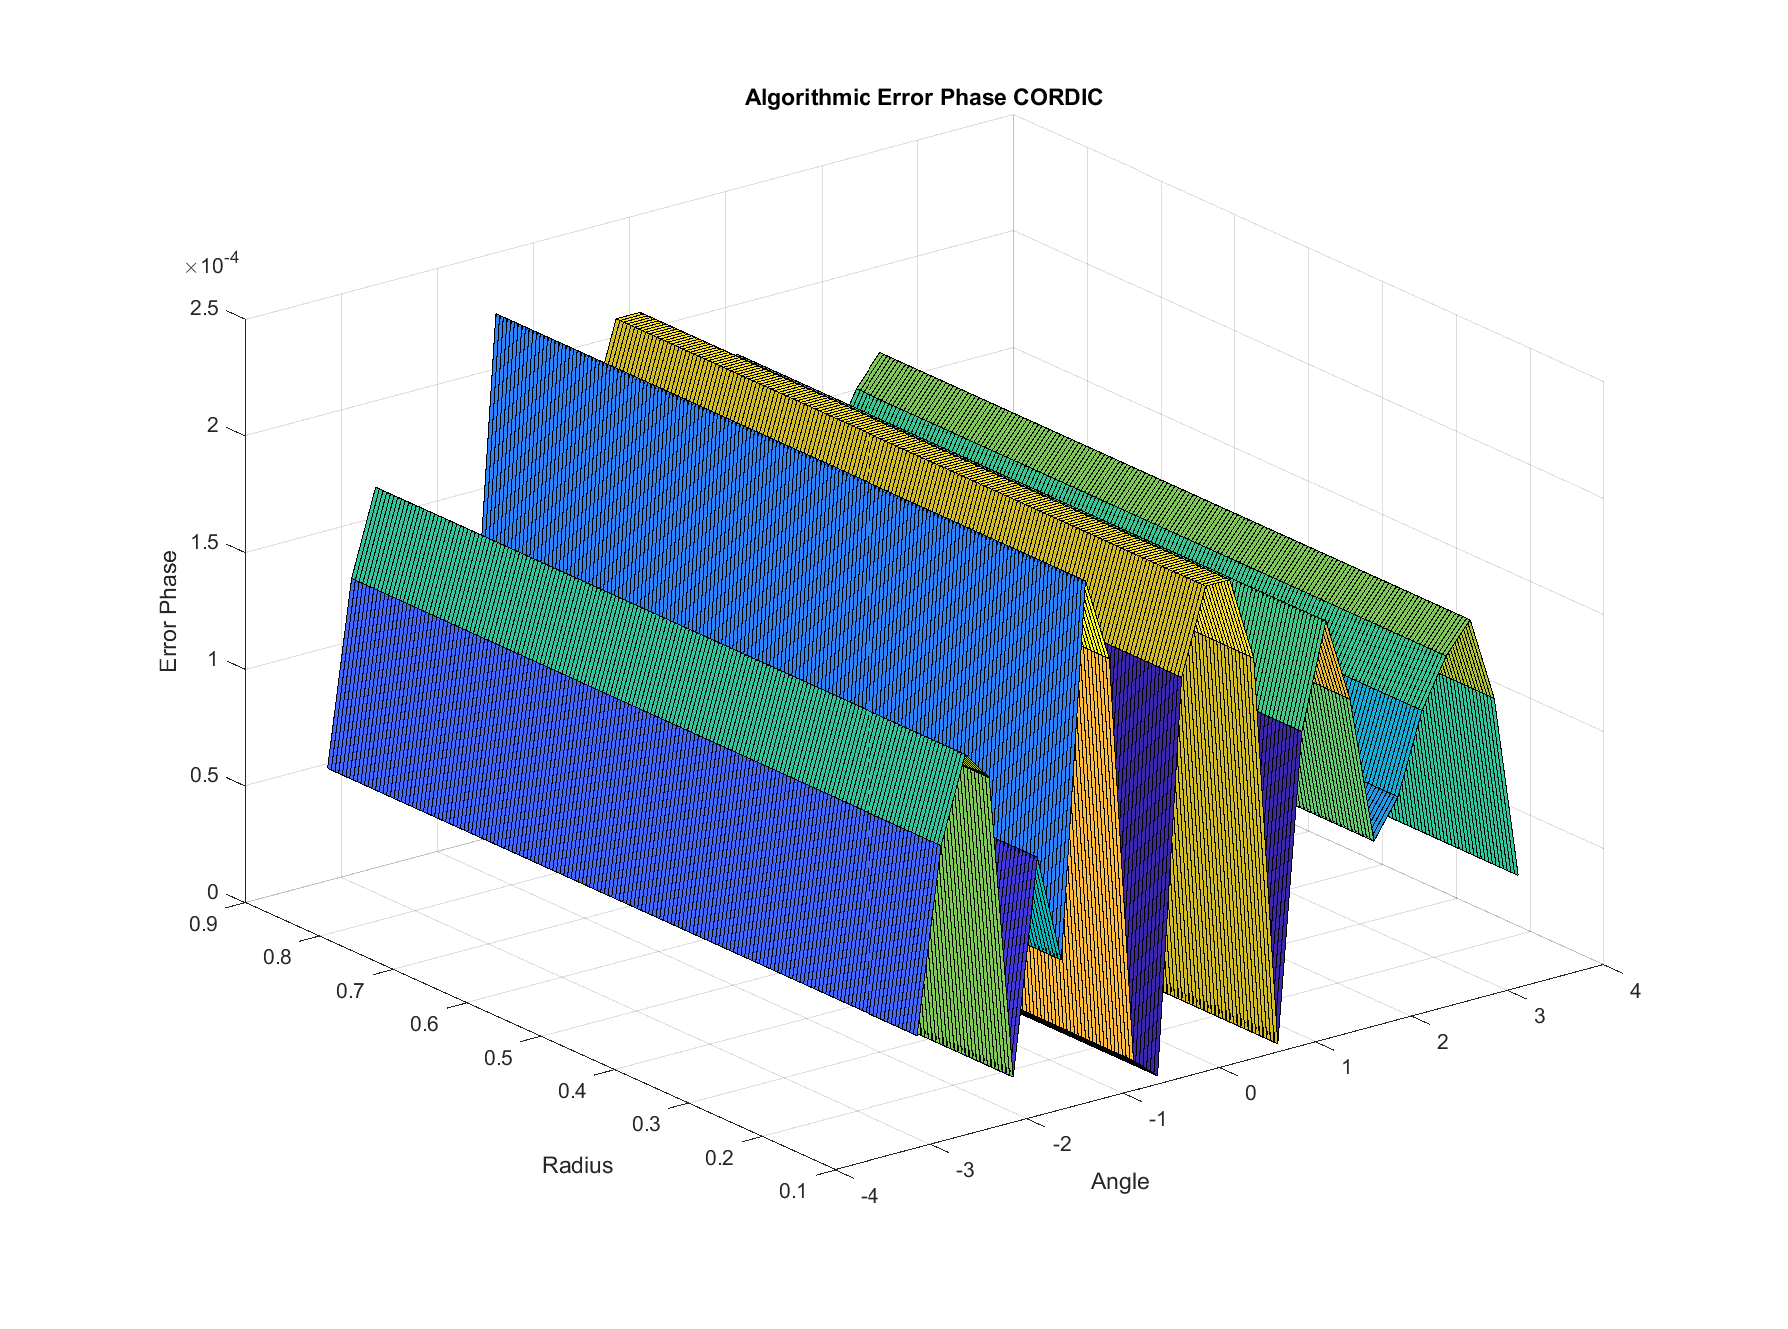
\includegraphics[width=\textwidth]{alg_error_phase}
	\caption{Algorithmic error Phase}\label{fig:floaterrorphase}
\end{figure}
\section{Quantized Model}
After the floating point model we moved towards lower level, performing a
quantization of input values. 

To do that we have to fix their dimensions in bits, that will be the same of the
VHDL implementation, after that we have to fix the range of acceptable x, y and
phase values so that we can compute the \emph{LSB} value for x, y and phase as
shown in \lstref{lst:cordicq}.

\lstinputlisting[language=matlab, label={lst:cordicq},
caption={CORDIC Quantized Model in Matlab 
(\code{cordic\_quantized.m}).}]{matlab/quantized/cordic_quantized.m}

The output of the test with the same input dataset, on this new quantized model
give us the opportunity to evaluate the quantization error introduced. In
\figref{fig:qerrorradius} we can appreciate the quantization error on the radius
and in \figref{fig:qerrorphase} on the phase.


\begin{figure}[ht]
	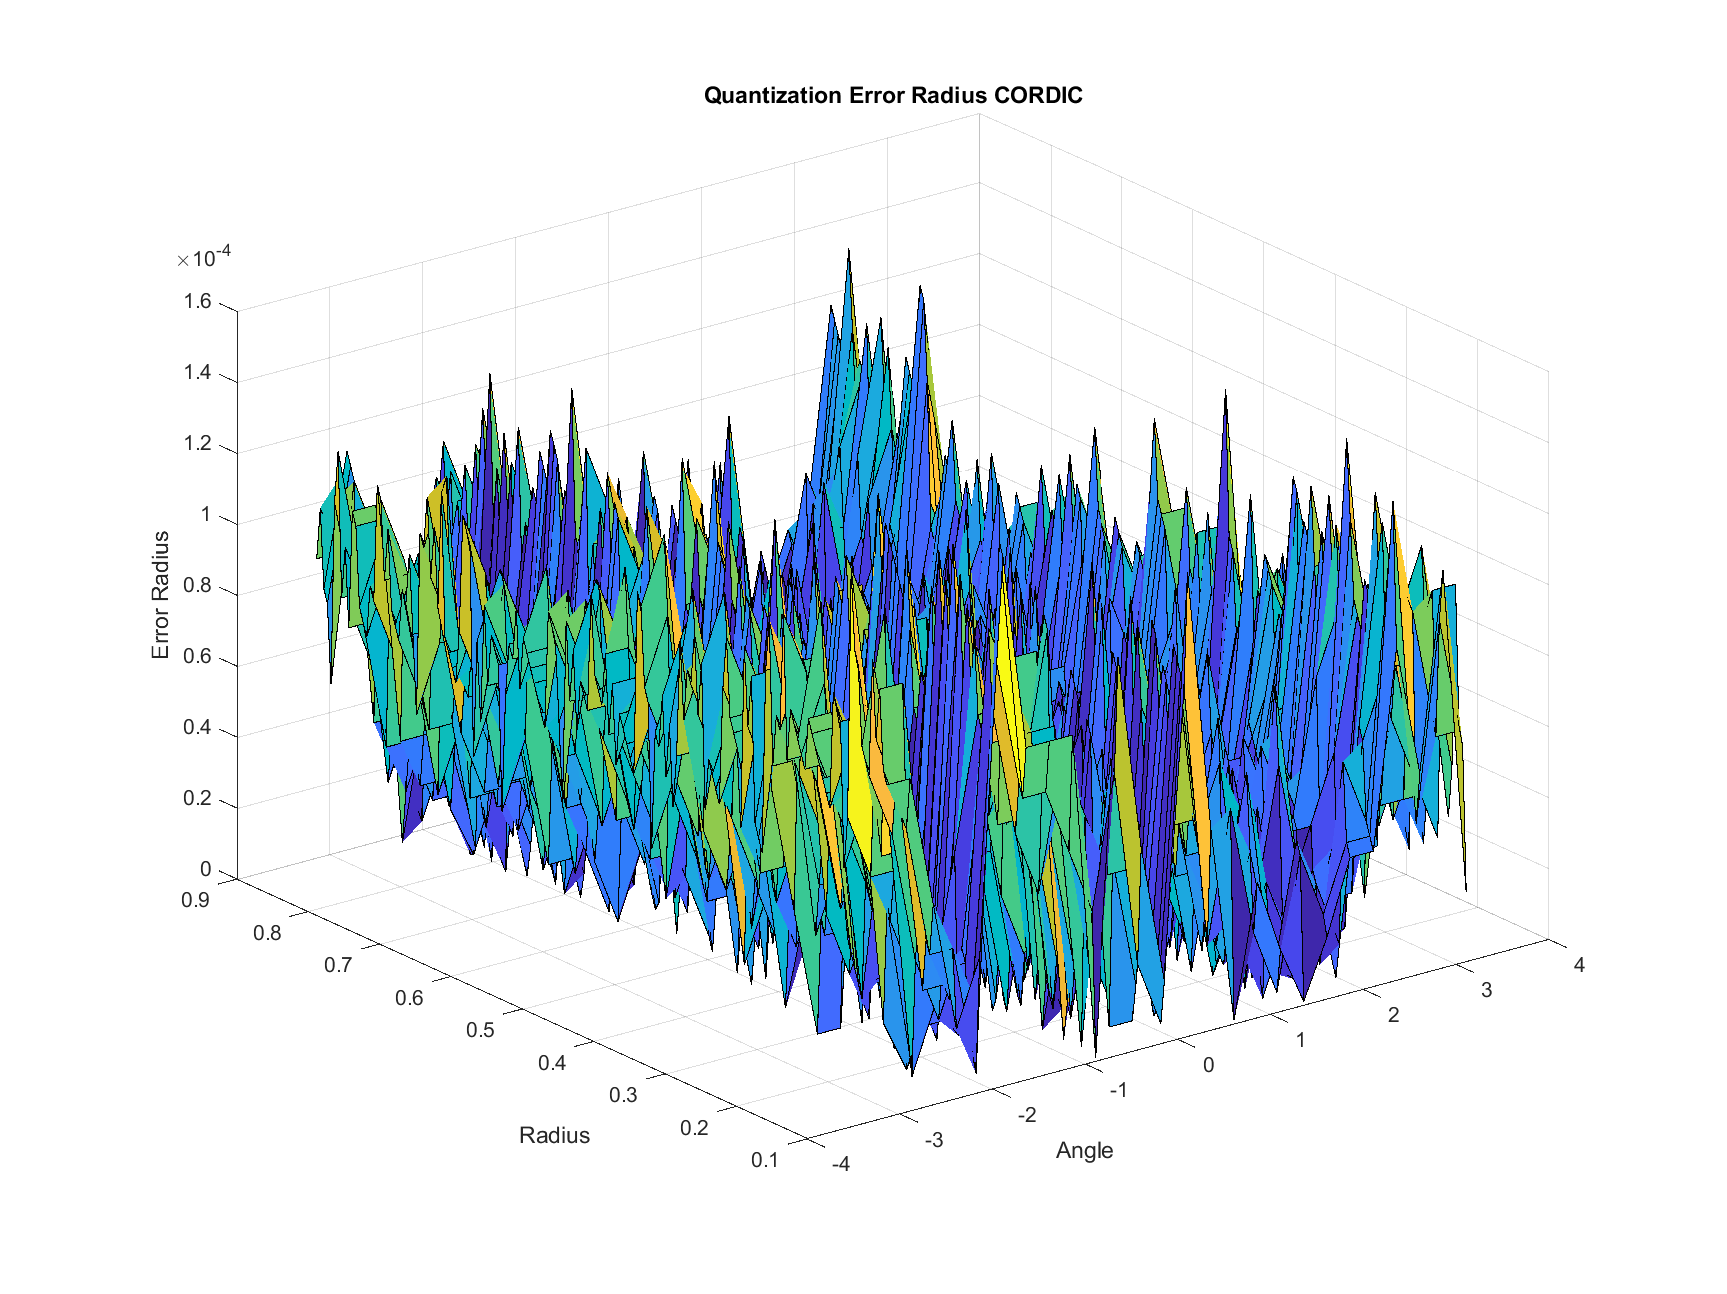
\includegraphics[width=\textwidth]{quant_error_radius}
	\caption{Quantization error Radius}\label{fig:qerrorradius}
\end{figure}
\begin{figure}[ht]
	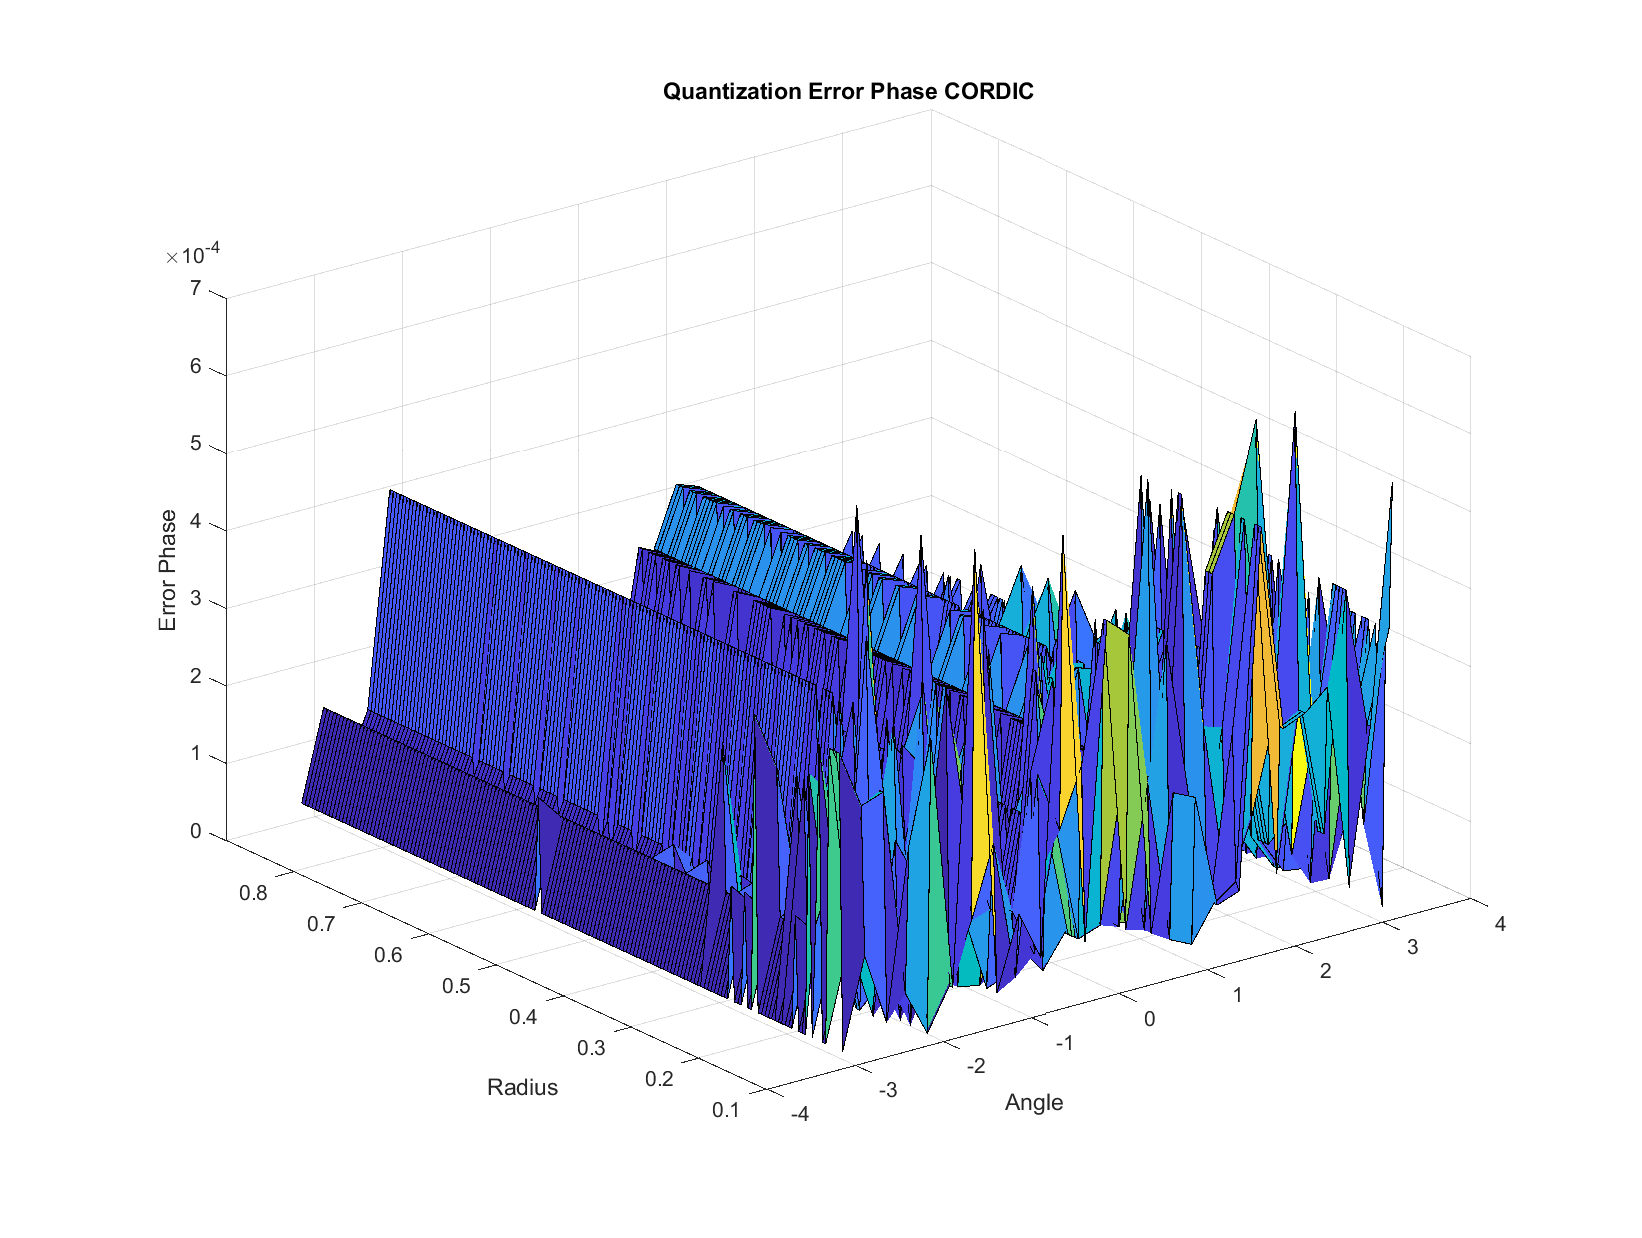
\includegraphics[width=\textwidth]{quant_error_phase}
	\caption{Quantization error Phase}\label{fig:qerrorphase}
\end{figure}
\section{VHDL model test}
The last step is to check te correctness of our implementation. To do that we
have to extract the output from the implementation through a simulation with
the testbench shown in \lstref{lst:testbench}.

\lstinputlisting[language=vhdl, label={lst:testbench},
caption={CORDIC testbench
(\code{cordic\_tb.vhd}).}]{CORDIC/hdl/tb/cordic_tb.vhd}


Then we can compute the error of the matlab model with respect to the
implementation. A correct implementation should have an output completely equal
to the quantized model's one.
The test performed in \lstref{lst:vhdloutputver} confirm that our implementation is
completely compliant with the \matlab model, thus is correct.

\lstinputlisting[language=matlab, label={lst:vhdloutputver},
caption={VHDL output verification in Matlab 
(\code{VHDL\_output\_verification.m}).}]{matlab/VHDL_output_verification.m}


